%%
%% 章:使ってみよう
%%------------------------------------------------------------------------------------------------------------------------------%%
\chapter{使ってみよう}
本章の第 1 節では、\LaTeX{}のインストールが不要な Web で\LaTeX{}を利用する方法を説明する。
第 2 節以降では、インストールと設定が完了しているパソコンで\LaTeX{}を使う方法を説明する。
%%
%% 節:Web で LaTeX を使う
%%--------------------------------------------------------------------------------------------------------------------%%
\section{Web で \LaTeX{}を使う}
今日では、パソコンに\TeX{}をインストールしなくても Web ブラウザ経由で\TeX{}を利用することができる。
Cloud LaTeX(https://cloudlatex.io)という本格的なサイトが存在するので、このサイトの利用を推奨する。
これ以外に ShareLaTeX(https://ja.sharelatex.com)や Overleaf(https://www.overleaf.com:旧 writeLaTeX)でも\XeLaTeX{}やLua\LaTeX{}により日本語の利用、IPAex フォントの埋め込みが可能である。\\

最初に Cloud LaTeX に新規登録(登録が完了していればログイン)する。\\

まずは新しいプロジェクトを作成する。
例えば「Test」という名前のプロジェクトを作成したとする。
プロジェクトに入ると「main.tex」というファイルがあるので、これに例えば次のように入力する。
\begin{quote}
\begin{verbatim}
\documentclass{jsarticle}
\begin{document}
アインシュタインは $E=mc^2$ と言った。
\end{document}
\end{verbatim}
\end{quote}
\vspc{-5.00pt}\begin{figure}[H]\centering\scalebox{0.25}{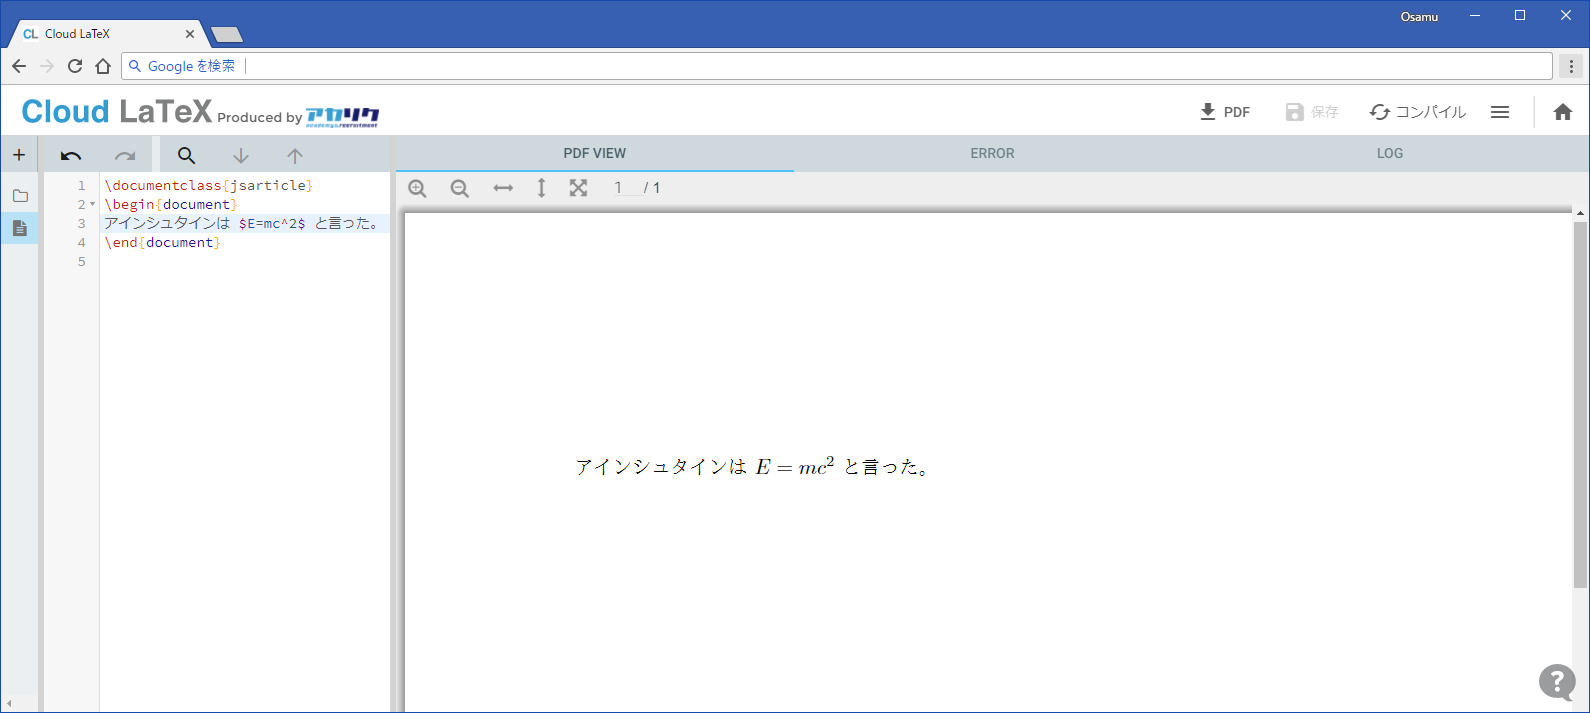
\includegraphics{./Fig/Fig02_01.PNG}}\end{figure}\vspc{-5.00pt}
自動コンパイルが有効になっていれば、PDF が作成され、右側にプレビューが表示される。
正しくコンパイルすることができたら PDF をダウンロードする。
正しくコンパイルすることができない場合には、右上の設定($\equiv$)をクリックして、LaTeX エンジンを「platex」に設定して「自動コンパイルを有効にする」をオフにしておき、必要に応じて「コンパイル」ボタンを押す方が軽快に作業することができる。
%%
%% 節:コマンドで行う方法
%%--------------------------------------------------------------------------------------------------------------------%%
\section{コマンドで行う方法}
Windows のコマンドプロンプトや PowerShell、Windows 上のオープンソースソフト Cygwin のシェル、Mac や Linux 等のターミナル上でコマンドを打ち込んで\LaTeX{}を利用する方法について説明する。
%%
%% 項:ターミナル(コマンドプロンプト・PowerShell)の起動
%%----------------------------------------------------------------------------------------------------------%%
\subsection{ターミナル(コマンドプロンプト・PowerShell)の起動}
Windows のコマンドプロンプトや PowerShell は、Cortana や検索ボックスに「コマンド(または cmd)」「PowerShell」と打ち込んで検索して実行することができる。
Cygwin をインストールした Windows の場合は mintty 等のターミナルを起動する。
Mac の「ターミナル」は「アプリケーション」→「ユーティリティ」の中に存在する。
以下では、これらをまとめて「ターミナル」と呼ぶことにする。\\

ターミナルを起動したら、まずは現在位置(カレントディレクトリ)に注意する。
必要に応じて cd コマンドでディレクトリを移動する。
%%
%% 項:エディタの起動
%%----------------------------------------------------------------------------------------------------------%%
\subsection{エディタの起動}
\LaTeX{}の文書ファイルを作成するには、テキストファイルを作成・編集するための「テキストエディタ」(単に「エディタ」とも言う)を用いる。\\

テキストエディタには多数の銘柄が存在する。
\TeX{}works や\TeX{}Shop の編集用のウィンドウもテキストエディタであり、Windows の「メモ帳(notepad)」や Mac の「テキストエディタ」は典型的なテキストエディタである。
Word などのワープロソフトもテキストエディタとして使うことができる(保存の際に「テキストファイル」形式を選択する)。\\

\TeX{}の文書ファイル名は、例えば ex1.tex のように\ruby{拡張子}{かくちょうし}(ファイル名の末尾)を tex にするのが一般的である。
以下では、ex1.tex という文書ファイルを作成し、それを\pLaTeX{}で処理してみることにする。\\

Windows の場合、ターミナルから
\vspc{+0.50zw}\begin{mdframed}[roundcorner=0.50zw,leftmargin=3.00zw,rightmargin=3.00zw,skipabove=0.40zw,skipbelow=0.40zw,innertopmargin=4.00pt,innerbottommargin=4.00pt,innerleftmargin=5.00pt,innerrightmargin=5.00pt,linecolor=gray!090,linewidth=0.50pt,backgroundcolor=gray!90]\color{gray!10}
\begin{verbatim}
notepad ex1.tex
\end{verbatim}
\end{mdframed}\vspc{-0.70zw}
のように打ち込むと「メモ帳」が起動する。「ファイル名 ex1.tex が見つかりません。新しく作成しますか?」と聞いてきたら[はい]と答える。\\

エディタを起動したら、最初は実験なので日本語は使わず、エディタの中に全て半角文字で次のように打ち込んでみる。
これは「Hello, \TeX{}!」という文と「$\textstyle{\int{}dx=x+C.}$」という数式を出力するための入力である。
\vspc{+0.50zw}\begin{mdframed}[roundcorner=0.50zw,leftmargin=3.00zw,rightmargin=3.00zw,skipabove=0.40zw,skipbelow=0.40zw,innertopmargin=4.00pt,innerbottommargin=4.00pt,innerleftmargin=5.00pt,innerrightmargin=5.00pt,linecolor=gray!020,linewidth=0.50pt,backgroundcolor=gray!20]
\begin{verbatim}
\documentclass{article}
\begin{document}
Hello,\TeX{}!
\[ \int dx = x + C. \]
\end{document}
\end{verbatim}
\end{mdframed}\vspc{-0.70zw}
打ち込み終わったら、エディタの起動時にファイル名を指定していない場合は ex1.tex というファイル名で保存する。
保存するフォルダ(ディレクトリ)は必ず先程のターミナルの現在位置と同じにしておかなければならない。
保存する際の文字コード(エンコーディング)は、従来の Windows ではシフト JIS が主流であったが、これからの時代は UTF-8 を推奨する。
\pLaTeX{}はシフト JIS、JIS(ISO-2022-JP)、EUC-JP、UTF-8 に対応している。
%%
%% 項:コマンドで LaTeX を起動する
%%----------------------------------------------------------------------------------------------------------%%
\subsection{コマンドで\LaTeX{}を起動する}
ex1.tex を\pLaTeX{}で処理するには、ターミナルに
\vspc{+0.50zw}\begin{mdframed}[roundcorner=0.50zw,leftmargin=3.00zw,rightmargin=3.00zw,skipabove=0.40zw,skipbelow=0.40zw,innertopmargin=4.00pt,innerbottommargin=4.00pt,innerleftmargin=5.00pt,innerrightmargin=5.00pt,linecolor=gray!090,linewidth=0.50pt,backgroundcolor=gray!90]\color{gray!10}
\begin{verbatim}
platex ex1.tex
\end{verbatim}
\end{mdframed}\vspc{-0.70zw}
と打ち込む。但し、デフォルトの文字コードはシステムによって異なる(自動判断するものも存在する)。
文字コードを例えば UTF-8 に指定して処理するには
\vspc{+0.50zw}\begin{mdframed}[roundcorner=0.50zw,leftmargin=3.00zw,rightmargin=3.00zw,skipabove=0.40zw,skipbelow=0.40zw,innertopmargin=4.00pt,innerbottommargin=4.00pt,innerleftmargin=5.00pt,innerrightmargin=5.00pt,linecolor=gray!090,linewidth=0.50pt,backgroundcolor=gray!90]\color{gray!10}
\begin{verbatim}
platex -kanji=utf8 ex1.tex
\end{verbatim}
\end{mdframed}\vspc{-0.70zw}
と打ち込む。utf8 の他に euc、jis、sjis を指定することができる。\\

ここで行ったことは、文書ファイル ex1.tex を dvi ファイル ex1.dvi に変換する作業\footnote{この作業を「タイプセットする」あるいは「コンパイルする」という。コンパイル(compile)とは、コンピュータのソースコード(テキストファイル)をオブジェクトコード(バイナリファイル)に変換する作業を指す言葉である。これらを\TeX{}の処理に当てはめて「\TeX{}ソース」を dvi ファイルあるいは PDF ファイルに変換する作業を「コンパイルする」という。} である。\\

なお、画面に ``No file ex1.aux.'' というメッセージが出る場合があるが、これはエラーメッセージではないので無視して構わない。
拡張子が aux のファイルは相互参照に使うもので、第 10 章で詳しく説明する。
同じファイルを再度\pLaTeX{}で処理すると、このメッセージは出なくなる。
エラーメッセージが出て止まってしまった場合は、後述の「エラーが発生した場合」を参照すること。\\

正常に終了したら、文書ファイル ex1.tex が格納されているフォルダに次の 3 つの新しいファイルが作成されているはずである。
\vspc{-0.50zw}\begin{itemize}\setlength{\leftskip}{1.90zw}%\setlength{\labelsep}{+1.00zw}
\item[\textbf{ex1.aux}:]
  aux ファイルもしくは補助(auxiliary)ファイルと呼ばれるもの。
  テキストファイルなので「メモ帳」などのテキストエディタで読むことができる。
  \LaTeX{}の「相互参照」という機能を使わない場合は何の意味も持たない。この場合、直ちに削除して構わない。
\item[\textbf{ex1.dvi}:]
  これが肝心の組版結果(dvi ファイル)である。
  このファイルに、どの文字をどのページのどの位置に配置するかという情報が書き込まれている。
  バイナリファイルなので通常のテキストエディタでは読むことはできない。
\item[\textbf{ex1.log}:]
  ログファイルと呼ばれるものである。
  実行の途中で画面に表示されるメッセージや、実行状態についての情報がここに書き込まれる。
  ログ(log)とは、航海日誌または一般に業務日誌を意味する英語である。
  テキストファイルなのでテキストエディタで読むことができる。
  エラーが生じた際に、その原因を調べるために用いるが、ここでは削除してしまって構わない。
\end{itemize}\vspc{-1.50zw}
%%
%% 項:PDF に変換する
%%----------------------------------------------------------------------------------------------------------%%
\subsection{PDF に変換する}
dvi ファイルを PDF ファイルに変換するには dvipdfmx というコマンドを用いる。
例えば、ex1.dvi を ex1.pdf に変換するには、ターミナルに次のように打ち込む\footnote{ここでは platex と dvipdfmx を順に実行したが、この 2 つをまとめて実行するコマンド ptex2pdf が存在する。ptex2pdf は「ptex2pdf -l ex1」のように用いる。}。
\vspc{+0.50zw}\begin{mdframed}[roundcorner=0.50zw,leftmargin=3.00zw,rightmargin=3.00zw,skipabove=0.40zw,skipbelow=0.40zw,innertopmargin=4.00pt,innerbottommargin=4.00pt,innerleftmargin=5.00pt,innerrightmargin=5.00pt,linecolor=gray!090,linewidth=0.50pt,backgroundcolor=gray!90]\color{gray!10}
\begin{verbatim}
dvipdfmx ex1
\end{verbatim}
\end{mdframed}\vspc{-0.70zw}
こうして生成された PDF ファイルは Adobe Reader でもプレビューすることができるが、Adobe Reader は重く、しかも開いている PDF をロックするので、PDF を生成する前に閉じなければならず効率が悪い。
\TeX{}Shop や\TeX{}works のような統合環境の PDF ビューアを使うか、あるいは単体の軽い PDF ビューアとして、Windows では SumatraPDF、Mac では OS X 付属の「プレビュー」などが使える。
これらは PDF ファイルをロックせず、PDF ファイルが更新されると自動的に再読み込みを行ってくれる。
%%
%% 節:日本語のテスト
%%--------------------------------------------------------------------------------------------------------------------%%
\section{日本語のテスト}
今度は日本語を入力して試してみる。
エディタで先程の文書ファイル ex1.tex を次のように適当に日本語を含めた形に書き直し、上書き保存する。
\vspc{+0.50zw}\begin{mdframed}[roundcorner=0.50zw,leftmargin=3.00zw,rightmargin=3.00zw,skipabove=0.40zw,skipbelow=0.40zw,innertopmargin=4.00pt,innerbottommargin=4.00pt,innerleftmargin=5.00pt,innerrightmargin=5.00pt,linecolor=gray!020,linewidth=0.50pt,backgroundcolor=gray!20]
\begin{verbatim}
\documentclass{jsarticle}
\begin{document}
こんにちは、\TeX{}!
\[ \int dx = x + 定数. \]
\end{document}
\end{verbatim}
\end{mdframed}\vspc{-0.70zw}
最初の行の article が jsarticle になる。
js を付けても付けなくても欧文・和文とも出力することができるが、標準の行間などが若干変化する。\enlargethispage{+0.30zw}
これを先程と同様に組版し、日本語部分も正しく表示できているかを確認する。もし、
\vspc{+0.50zw}\begin{mdframed}[roundcorner=0.50zw,leftmargin=3.00zw,rightmargin=3.00zw,skipabove=0.40zw,skipbelow=0.40zw,innertopmargin=4.00pt,innerbottommargin=4.00pt,innerleftmargin=5.00pt,innerrightmargin=5.00pt,linecolor=gray!090,linewidth=0.50pt,backgroundcolor=gray!90]\color{gray!10}
\begin{verbatim}
! LaTeX Error: This file needs format 'pLaTeX2e'
               but this is 'LaTeX2e'.
\end{verbatim}
\end{mdframed}\vspc{-0.70zw}
などと言って止まってしまうなら、\TeX{}の設定が間違っていて英語版 \LaTeX(\pdfLaTeX{}など)を呼び出してしまっている可能性がある。\\

\pLaTeX{}や dvipdfmx の処理が正常に終わっても、PDF ビューアに日本語部分が表示されない場合は、日本語フォントを埋め込む設定がうまくできていないことが考えられる。
設定を見直しても改善しないようなら、PDF ビューアが使用している環境に合わないことも考えられるので、別の PDF ビューアを試してみるとよい。
%%
%% 節:SyncTeX の使い方
%%--------------------------------------------------------------------------------------------------------------------%%
\section{Sync\TeX{}の使い方}
Sync\TeX{}はエディタ(\TeX{}ソース編集画面)と PDF プレビュー画面との相互リンクのための仕組みである。
\TeX{}works や\TeX{}Shop のような統合環境の他、PDF ビューアでは SumatraPDF、エディタでは Emacs などが対応している。\\

例えば、\TeX{}works ではエディタの画面を Ctrl+左クリックすると PDF の該当箇所にジャンプし、逆に PDF の画面を Ctrl+左クリックするとソースの該当箇所にジャンプする。\\

\TeX{}側でも Sync\TeX{}に対応している必要がある。
\pdfTeX{}や W32\TeX{}の\pTeX{}では以前から対応していたが、現在は Windows 版以外の\pTeX{}でも対応している。
これらの\TeX{}を起動するコマンドに -synctex=1 オプションを付ければ Sync\TeX{}が有効になる。\\

SumatraPDF のサイトには、SumatraPDF と Emacs(AUC\TeX)などのエディタを組み合わせて Sync\TeX{}を動作させる方法が詳しく記載されている。\\

Sync\TeX{}の仕組みは、\TeX{}側が入力・出力の位置の対応関係を「ファイル名.synctex.gz」という圧縮ファイルに書き出すだけである。
PDF ファイルに余計な情報が挿入されることはない。
%%
%% 節:TeX2img の紹介
%%--------------------------------------------------------------------------------------------------------------------%%
\section{TeX2img の紹介}
寺田侑祐{\small 氏}(Windows 版は安倍紀行{\small 氏})作の TeX2img は、\LaTeX{}出力を画像に変換するためのツールである。
PDF、EPS、PNG、SVG、EMF など多様な画像形式をサポートしている。
\LaTeX{}で出力した数式を別のソフト(DTP ソフト、ワープロソフト、プレゼンソフト等)や Web ページに貼り付けたりするために便利である。
Mac 版、Windows 版が存在する。
使い方は、\LaTeX{}ソースを貼り付けて「画像生成」ボタンを押すだけである。\\

詳しくは、TeX2img 配布サイト\footnote{https://tex2img.tech/}を参照のこと。
%%
%% 節:エラーが発生した場合
%%--------------------------------------------------------------------------------------------------------------------%%
\section{エラーが発生した場合}
本稿に登場する数行の例でも、あるいはもっと長い雛形でも、とにかく確実にタイプセットできる例を出発点として、1 つずつ新しい技を覚えていくこと。
始めのうちは、1 つ命令を追加したら直ちにタイプセットしてみることを推奨する。
そうすれば、どこでエラーが発生したのか自ずと分かるだろう。\\

\verb`\` で始まる命令の綴りを間違えた場合、エラーメッセージが現れ、入力待ちの状態となる。\\

メッセージ ``! Undefined control sequence.'' は、未定義(undefined)の命令(control sequence)が使われているという意味である。
エラーが発生した際、次の処理を選ぶことができる。
\vspc{-0.50zw}\begin{itemize}\setlength{\leftskip}{-1.00zw}%\setlength{\labelsep}{+1.00zw}
\item そのまま Enter を押せば、エラーを無視して処理を続行する。うまく行けばエラー箇所以外の処理ができるかもしれない。
\item x(エックス)を入力して Enter を押せば\LaTeX{}による処理を中断する。\TeX{}works では dvipdfmx による処理に移行するので、うまく行けばエラーの少し前までの PDF 出力が得られるかもしれない。x は e\underline{x}it(終了)を意味する(間違えて quit のつもりで q を打つと、エラーを表示せずに続行する quiet モードになってしまう)。
\end{itemize}\vspc{-1.50zw}
%%
%% 項:不明なエラーが発生した場合
%%----------------------------------------------------------------------------------------------------------%%
\subsection{不明なエラーが発生した場合}
もし原因不明のエラーが発生して、対処法が分からない場合は、まずはエラーメッセージを Google などで検索してみるとよい。
大抵、何らかのヒントが得られるだろう。\\

それでも分からない場合は、質問用掲示板にて質問する。\\

もっとも「インストールしたけれど動きません。どうしたらいいですか?」といった質問では、誰も答えてくれないだろう。
例えば「Windows 10 に『美文書第 7 版』DVD からインストールした\TeX~Live 2016 で、\TeX{}works に○ページの例を入力して[タイプセット]ボタンを押すと次のようなエラーメッセージが出ます」といった具体的な質問であれば、そのとき時間のある有志の方が答えてくれるだろう。\\

肝心なのは、エラーが再現できる材料を全て提示することである。
但し、もし何百行もあるファイルでエラーが発生したなら、それを全て送るのではなく、本質的でない部分を少しずつ削って短くし、これ以上短くするとエラーが発生しなくなる(あるいは別のエラーが発生する)ところまで短くして添付すること。
これがいわゆる「エラーが再現する最小例」である。
厳密に「最小」である必要はないが、このようにエラーを保ったままファイルを切り詰めることで、エラーの原因が自ずと明らかになることが多々ある。
%%
%% 節:texdoc の使い方
%%--------------------------------------------------------------------------------------------------------------------%%
\section{texdoc の使い方}
\TeX~Live のマニュアルは「texdoc」というコマンドで参照することができる。
例えば、jsarticle の詳しい使い方を知りたければ、ターミナル上に次のように打ち込む。
\vspc{+0.50zw}\begin{mdframed}[roundcorner=0.50zw,leftmargin=3.00zw,rightmargin=3.00zw,skipabove=0.40zw,skipbelow=0.40zw,innertopmargin=4.00pt,innerbottommargin=4.00pt,innerleftmargin=5.00pt,innerrightmargin=5.00pt,linecolor=gray!090,linewidth=0.50pt,backgroundcolor=gray!90]\color{gray!10}
\begin{verbatim}
texdoc jsarticle
\end{verbatim}
\end{mdframed}\vspc{-0.70zw}
これで「\pLaTeXe{}新ドキュメントクラス」というマニュアルが画面に表示される。
``texdoc jsarticle'' だけでなく ``texdoc jsbook'' や ``texdoc jsclasses'' と打ち込んでも同じマニュアルが表示される\footnote{texdoc は候補となるマニュアルのファイル名などを元にもっともらしさの点数を付け、最高得点のマニュアルを 1 つ開く。検討対象になった他のマニュアルも参照したい場合には、\texttt{texdoc -l} で一覧から指定することができる。}。
